\documentclass{report}

\input{~/dev/latex/template/preamble.tex}
\input{~/dev/latex/template/macros.tex}

\title{\Huge{Calculus 1, Chapter 4 Notes}}
\author{\huge{Nathan Warner}}
\date{\huge{Started March 26, 2023}}
\pagestyle{fancy}
\fancyhf{}
\rhead{MATHEMATICS NOTES}
\lhead{\leftmark}
\cfoot{\thepage}
\graphicspath{{./images}}
% \usepackage[default]{sourcecodepro}
% \usepackage[T1]{fontenc}

\pgfpagesdeclarelayout{boxed}
{
  \edef\pgfpageoptionborder{0pt}
}
{
  \pgfpagesphysicalpageoptions
  {%
    logical pages=1,%
  }
  \pgfpageslogicalpageoptions{1}
  {
    border code=\pgfsetlinewidth{1.5pt}\pgfstroke,%
    border shrink=\pgfpageoptionborder,%
    resized width=.95\pgfphysicalwidth,%
    resized height=.95\pgfphysicalheight,%
    center=\pgfpoint{.5\pgfphysicalwidth}{.5\pgfphysicalheight}%
  }%
}

\pgfpagesuselayout{boxed}

\begin{document}
    \maketitle
    \begin{center}
        \begin{Huge}
            \textbf{Chapter 4}
        \end{Huge}
    \end{center}
    \line(1,0){490}
    \bigbreak \noindent \bigbreak \noindent  
    \begin{Huge}
        \noindent \textbf{Contents}
    \end{Huge}
    \bigbreak \noindent
    \begin{Large}
        \bigbreak \noindent 
        \textbf{\noindent 4.1: Maximum and Minimum Values (2-7)}
        \bigbreak \noindent \bigbreak \noindent 
        \textbf{4.2: The Mean Value Theorem}
        \bigbreak \noindent \bigbreak \noindent 
        \textbf{4.3: How Derivatives Affect the Shape of a Graph}
        \bigbreak \noindent \bigbreak \noindent 
        \textbf{4.4: Indeterminate Forms and L'Hospital's rule}
        \bigbreak \noindent \bigbreak \noindent 
        \textbf{4.5: Summary of Curve Sketching}
        \bigbreak \noindent \bigbreak \noindent 
        \textbf{4.7: Optimization Problems}
        \bigbreak \noindent \bigbreak \noindent 
        \textbf{4.8: Newton's Method}
        \bigbreak \noindent \bigbreak \noindent 
        \textbf{4.9: Antiderivatives}
    \end{Large}
    \pagebreak \bigbreak \noindent

    \begin{Large}
        \begin{mdframed}
            \begin{center}
                \textbf{4.1}
            \end{center}
        \end{mdframed}
    \end{Large}
    \begin{Large}
        \begin{center}
            \textbf{Maximum and Minimum Values}
        \end{center}
    \end{Large}
    \line(1,0){490}
    
    \bigbreak \noindent \bigbreak \noindent \bigbreak \noindent 
    We will examine how derivatives affect the shape of a graph of a function 
    and how they help us locate the maximum and minimum values.

    \smallbreak \noindent
    \begin{mdframed}
      \textbf{\textit{\underline{Absolute Maximum:}}}
      A function $f$ has an absolute maximum at  $c$ if $f(c) \geq f(x)$ for all $x \in$ Domain of $f$
      \bigbreak \noindent 
      \textbf{\textit{\underline{Absolute Minimum:}}}
      A function $f$ has an absolute minimum at $k$ if  $f(c) \leq f(x)$ for all  $x \in$ Domain of  $f$
       \bigbreak \noindent 
      \textbf{\textit{\underline{Local (Relative) Maximum}}}
      A function $f$ has a local maximum at  $b$ if  $f(b) \geq f(x)$ when  $x$ is near  $b$
      \bigbreak \noindent 
      \textbf{\textit{\underline{Local (Relative) Minimum}}}
      A function $f$ has a local minimum at  $m$ if  $f(m) \leq f(x)$ when  $x$ is near  $m$
    \end{mdframed}

    \bigbreak \noindent 
    \begin{center}
      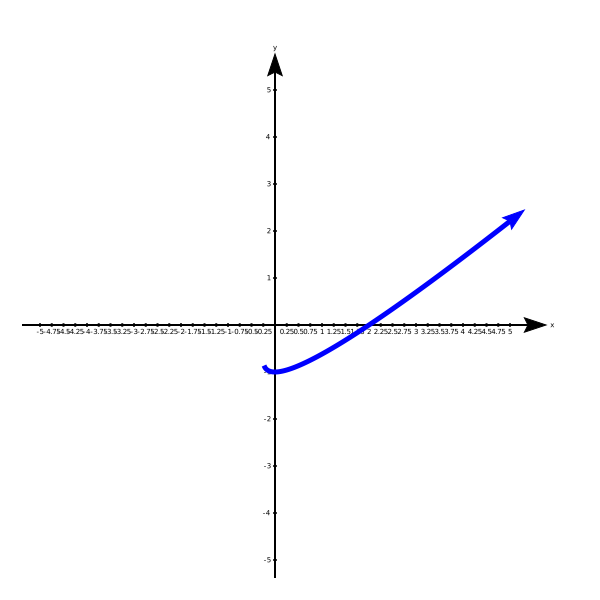
\includegraphics[scale=0.5]{ ./images/1.png }
    \end{center}

    \bigbreak \noindent 
    \nt{Endpoints are \textbf{\textit{\underline{Not}}} considered \textbf{\textit{\underline{local}}} max/min values.}

    \bigbreak \noindent 
    \begin{mdframed}
      \textbf{Example: Sketch the graph of $f$ to find the absolute and local max and min (extrema) values of $f$}
      \begin{align*}
        f(x) = 1+(x+1)^{2},\ -2\leq x < 2
      .\end{align*}
    \end{mdframed}

    \pagebreak \bigbreak \noindent
    \textit{Gather Points:}
    \begin{align*}
      f(-2) = 1+ (-2 + 1)^{2} = 2 \\
      f(-1) = 1 \\
      f(0) = 2 \\
      f(1) = 5 \\
      f(2) = 10
    .\end{align*}

    \bigbreak \noindent 
    \textit{Graph:}
    \begin{center}
      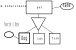
\includegraphics[scale=0.8]{ ./images/2.png}
    \end{center}

    \bigbreak \noindent 
    \nt{No arrows because of the restriction, and open circle on (2,10) because of the restriction}

    \bigbreak \noindent 
    \begin{center}
      Absolute Max: None \\
      Absolute Min: f(-1) = 1\\
      Local Max: None \\
      Local Min: f(-1) = 1
    \end{center}

    \bigbreak \noindent 
    \begin{mdframed}
      \textbf{Extreme Value Theorem:}
      If $f$ is continuous on a closed interval [a,b], then $f$ attains an
      obsulute maximum value $f(c)$ and an absolute minimum value $f(d)$ where $c,d \in [a,b]$
    \end{mdframed}

    \smallbreak \noindent
    \begin{mdframed}
      \textbf{Fermat's Theorem:}
      If $f$ has a local minimum or maximum at $c$, and if $f^{\prime}(c)$ exists, 
      then $f^{\prime}(c)=0$
    \end{mdframed}

    \smallbreak \noindent
    \begin{mdframed}
      \textbf{Critical Number:}
      $c$ in the domain of $f(x)$ is a critical number if $f^{\prime}(c)=0$ or if $f^{\prime}(c)$ does not exist. \\
      Note: If $f$ has a local max or min at $c$, then $c$ is a critical number of $f$ 
    \end{mdframed}

    \pagebreak \bigbreak \noindent
    \begin{mdframed}
      \textbf{Example: Find the critical numbers of:}
      \begin{align*}
        h(p) = \frac{p-1}{p^{2}+4}
      .\end{align*}
      \textit{So: Find $h^{\prime}(p)$ and solve $h^{\prime}(p)=0$ and $h^{\prime}(p)$ DNE}
    \end{mdframed}

    \bigbreak \noindent
    \textit{So:}
    \begin{align*}
      h^{\prime}(p) = \frac{(p^{2}+4)(1) - (p-1)(2p)}{(p^{2}+4)^{2}} \\
      = \frac{p^{2}+4-2p^{2}+2p}{(p^{2}+4)^{2}} \\
      = \boxed{\frac{-p^{2}+2p+4}{(p^{2}+4)^{2}}}
    \end{align*}

    \bigbreak \noindent 
    \textit{$h^{\prime}(p)= 0$}
    \begin{align*}
      -p^{2} + 2p + 4 = 0 \\
      p^{2}-2p-4 =0 
    .\end{align*}

    \bigbreak \noindent 
    \textit{This does not factor so we will use the quadratic formula:}
    \begin{align*}
      \frac{2\pm \sqrt{(-2)^{2} -4(1)(-4)}}{2(1)} \\
      = \frac{2 \pm \sqrt{20}}{2} \\
      \frac{2\pm 2 \sqrt{5}}{2} \\ 
      = \boxed{1\pm \sqrt{5}}
    .\end{align*}

    \bigbreak \noindent 
    \textit{Find where $h^{\prime}(p)$ DNE}
    \begin{align*}
      (p^{2} +4)^{2} = 0 \\
      p^{2} + 4 = 0 \\
      p^{2} = -4 \\
      \boxed{None}
    .\end{align*}

    \pagebreak \bigbreak \noindent
    \begin{large}
      \begin{center}
        \textbf{How to find the absolute maximum and minimum values of a continuous function $f$ on a closed interval [a,b]}
      \end{center}
    \end{large}

    \bigbreak \noindent 
    \begin{enumerate}
      \item Find critical values of f in (a,b)
      \item Find $f(a)$ and $f(b)$
      \item Absolute Max: largest from 1.) and 2.) 
      \item Absolute Min: smallest from 1.) and 2.)
    \end{enumerate}

    \bigbreak \noindent 
    \begin{mdframed}
      \textbf{Example: Find the absolute max and min values of:}
      \begin{align*}
        f(x) = (x^{2} - 1)^{3}\ \text{on}\ \ [-1,2]
      .\end{align*}
    \end{mdframed}

    \bigbreak \noindent
    \textit{So:}
    \begin{align*}
      f^{\prime}(x) = 3(x^{2} -1)^{2} \cdot 2x \\
      = 6x(x^{2} -1)^{2}\\
    \end{align*}

    \bigbreak \noindent 
    \textit{1.) Find Critical Values:}

    \bigbreak \noindent 
    \textbf{\textit{\underline{$f^{\prime}(x) = 0$}}}
    \begin{align*}
      6x(x^{2} -1)^{2} = 0 \\
    .\end{align*}
    \begin{align*}
      6x = 0 \\
      x = 0
    .\end{align*}
    \begin{align*}
      (x^{2} -1)^{3} = 0 \\
      x^{2} - 1 = 0  \\
      x = \pm 1
    .\end{align*}

    \bigbreak \noindent 
    \textbf{\textit{\underline{$f^{\prime}(x)$ DNE}}}
    \begin{center}
      None
    \end{center}

    \bigbreak \noindent 
    \textbf{\textit{\underline{Therefore:}}}
    \begin{center}
      Critical Numbers: $x=-1,1,0$
    \end{center}

    \bigbreak \noindent \bigbreak \noindent 
    \textit{Now plug these into f(x):}
    \begin{align*}
      f(-1) = 0 \\
      f(1) = 0 \\
      f(0) = -1
    .\end{align*}

    \pagebreak \bigbreak \noindent
    \textit{2.) Find $f(a)$ and $f(b)$}
    \begin{align*}
      f(a) = f(-1) = 0 \\
      f(b) = f(2) = (2^{2} -1)^{3} \\
      = 27
    .\end{align*}

    \bigbreak \noindent 
    \textit{3.) Find abs max and abs min:}
    \begin{align*}
      \text{Abs max: } f(2) = 27 \\
      \text{Abs min: } f(0) = -1
    .\end{align*}

    \bigbreak \noindent 
    \begin{mdframed}
      \textbf{Example: Find the abs max and min of:}
      \begin{align*}
        f(t) = t\sqrt{25-t^{2}}\ on\ [-1,5]
      .\end{align*}
    \end{mdframed}

    \bigbreak \noindent
    \textit{So:}
    \begin{align*}
      f^{\prime}(t) = t(25-t^{2})^{\frac{1}{2}} \\
      = (1)(25-t^{2})^{\frac{1}{2}} + (t)\bigg(\frac{-t}{2(25-t^{2})^{\frac{1}{2}}}\bigg) \\
      = (25-t^{2})^{\frac{1}{2}} + \bigg(\frac{-2t^{2}}{2(25-t^{2})^{\frac{1}{2}}}\bigg) \\
      = (25-t^{2})^{\frac{1}{2}} + \bigg(\frac{-t^{2}}{(25-t^{2})^{\frac{1}{2}}}\bigg) \\
      =\frac{-t^{2} + 25 - t^{2}}{(25-t^{2})^{\frac{1}{2}}} \\
      = \frac{25-2t^{2}}{\sqrt{25-t^{2}}}
    \end{align*}

    \bigbreak \noindent 
    \textit{1.) Find critial values:} 
    \bigbreak \noindent 
    \textit{Set numerator = 0:}
    \begin{align*}
      25-2t^{2}=  0 \\ 
      25 = 2^{2} \\
      t^{2} = \frac{25}{2} \\
      t = \pm \frac{5}{\sqrt{2}}
    .\end{align*}

    \bigbreak \noindent 
    \nt{Since $- \frac{5}{\sqrt{2}}$ is smaller than the lower bound in interval, the only critical value we have is $\frac{5}{\sqrt{2}}$}

    \bigbreak \noindent 
    \textit{Eval $\frac{5}{\sqrt{2}}$:}
    \begin{align*}
      f(\frac{5}{\sqrt{2}}) = \frac{5}{\sqrt{2}}\sqrt{25-\frac{25}{2}} \\
      = \frac{5}{\sqrt{2}}\sqrt{\frac{25}{2}} \\
      = \frac{5}{\sqrt{2}} \cdot \frac{5}{\sqrt{2}} \\
      = \boxed{\frac{25}{2}}
    .\end{align*}

    \bigbreak \noindent 
    \textit{$f^{\prime}(t) DNE$}
    \begin{align*}
      25-t^{2} \leq 0 \\ 
      (5 - t)(5+t) \leq 0
    .\end{align*}

   \bigbreak \noindent 
   \begin{center}
     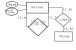
\includegraphics[scale=1]{ ./images/3.png }
   \end{center}

   \bigbreak \noindent 
   \begin{align*}
     DNE\ (-\infty, -5] \cup [5, \infty]
   .\end{align*}

   \bigbreak \noindent 
   \textit{But if we consider the interval [-1,5], then the only critical number that is within this interval is:}
   \begin{align*}
     5
   .\end{align*}

   \bigbreak \noindent
   \textit{So:}
   \begin{align*}
     f(5) = 5\sqrt{25-5^{2}} \\
     = \boxed{0}
   \end{align*}

   \bigbreak \noindent 
   \textit{2.) Eval at -1 and 5:}
   \begin{align*}
     f(-1) = -\sqrt{24} \\
     = -2\sqrt{6} \\
     \approx \boxed{-4.899}
   .\end{align*}
   \begin{align*}
     f(5) = \boxed{0}
   .\end{align*}

   \bigbreak \noindent 
   \textit{3.) Compare and find abs max and min:}
   \begin{align*}
     \text{Abs max: } f(\frac{5}{\sqrt{2}}) = \frac{25}{2} \\
     \text{Abs min: } f(-1) = -2\sqrt{6}
   .\end{align*}

   \bigbreak \noindent 
   \nt{It is possible to have more than 1 abs max value if they are the same y value.}

   \pagebreak \bigbreak \noindent
   \begin{Large}
       \begin{mdframed}
           \begin{center}
               \textbf{4.2}
           \end{center}
       \end{mdframed}
   \end{Large}
   \begin{Large}
       \begin{center}
           \textbf{The Mean Value Theorem}
       \end{center}
   \end{Large}
   \line(1,0){490}

   \bigbreak \noindent 
   \begin{mdframed}
     \textbf{Rolle's Theorem:}
     \bigbreak \noindent 
     If f(x) satisfies the following:
     \begin{enumerate}
       \item continuous on [a,b]
        \item differentiable on (a,b)
        \item f(a) = f(b)
     \end{enumerate}
     \smallbreak \noindent
     Then there is a $c \in (a,b)$ such that $f^{\prime}(c) = 0$ 
   \end{mdframed}

   \bigbreak \noindent 
   \begin{mdframed}
     \textbf{Example: verify that f(x) satisfies the conditions of Rolle's Theorem, then find all 
       numbers c that satisfy the conclusion
     }
     \begin{align*}
       f(x) = x^{3} -x^{2} -6x + 2,\ in\ [0,3]
     .\end{align*}
   \end{mdframed}

   \bigbreak \noindent
   \textit{So:}
   \begin{enumerate}
     \item f(x) is continuous on [0,3] because it's a polynomial
      \item f(x) is differentiable on (0,3) because it's a polynomial
      \item f(a) ?= f(b)
   \end{enumerate}

   \bigbreak \noindent 
   \textit{3.)}
   \begin{align*}
     f(0) = 2 \\
      f(3) = 2
   .\end{align*}

   \bigbreak \noindent 
   \textit{So step 3 passes.}

   \bigbreak \noindent 
   \textbf{\textit{\underline{Find all $c \in (0,3) $ such that $f^{\prime}(c) = 0$}}}
   \begin{align*}
     f^{\prime}(c) = 3c^{2} - 2c - 6 
   .\end{align*}

   \bigbreak \noindent 
   \textit{Now set that equal to 0}
   \begin{align*}
     3c^{2} -2c - 6 = 0
   .\end{align*}

   \bigbreak \noindent 
   \textit{does not factor so use quadratic formula}
   \begin{align*}
     c = \frac{2\pm\sqrt{(-2)^{2} - 4(3)(-6)}}{2(3)} \\
     =\frac{2\pm\sqrt{76}}{6} \\
     = \frac{2\pm 2\sqrt{19}}{6} \\
     = \frac{1\pm \sqrt{19}}{3}
   .\end{align*}

   \bigbreak \noindent 
   \textit{Only use positive version because of the interval}

   \bigbreak \noindent 
   \textbf{\textit{\underline{Therefore}}}
   \begin{align*}
     c = \frac{1+\sqrt{19}}{3}\\
     \approx 1.7
   .\end{align*}

   \bigbreak \noindent 
   \begin{mdframed}
     \textbf{The mean value theorem:}
     \bigbreak \noindent 
     if f(x) satisfies the following:
     \begin{enumerate}
       \item continuous on [a,b]
        \item differentiable on (a,b)
     \end{enumerate}
     \smallbreak \noindent
     then there is a number $c \in (a,b)$ such that
     \begin{align*}
       f^{\prime}(c) = \frac{f(b) - f(a)}{b -a}
     .\end{align*}
   \end{mdframed}

   \bigbreak \noindent 
   \begin{mdframed}
     \textbf{Example: verify that f(x) satisfies the conditions of the mean value theorem, then 
       find all the numbers c that satisfy the conclusion
     }
     \begin{align*}
       f(x) = \frac{x}{x+2},\ [1,4]
     .\end{align*}
   \end{mdframed}

   \bigbreak \noindent 
   \begin{enumerate}
     \item f(x) is continuous on [1,4] because f is a rational function, undefined at x = -2 $\notin [1,4]$
      \item f(x) is differentiable on (1,4)
   \end{enumerate}

   \bigbreak \noindent 
   \textit{2.)}
   \begin{align*}
     f^{\prime}(x) = \frac{(x+2)(1) - (x)(1)}{(x+2)^{2}} \\
     = \frac{2}{(x+2)^{2}}
   .\end{align*}

   \bigbreak \noindent 
   \textit{We can see that $f^{\prime}(x)$ would be undefined at -2, but that's not a problem because -2 is not in the interval}

   \bigbreak \noindent 
   \textbf{\textit{\underline{Therefore:}}} $f^{\prime}(x)$ is defined on (1,4) so it is differentiable on (1,4)

   \bigbreak \noindent 
   \textbf{\textit{\underline{Find all c such that $f^{\prime}(c) = \frac{f(b) - f(a)}{b-a}$}}}

   \bigbreak \noindent
   \textit{So:}
   \begin{align*}
    \frac{f(4) - f(1)}{4-1} \\
    = \frac{\frac{4}{6} - \frac{1}{3}}{4-1} \\
    = \frac{\frac{1}{3}}{3} \\ 
    = \frac{1}{9}
   \end{align*}

   \bigbreak \noindent 
   \textit{Set $f^{\prime}(c) = \frac{1}{9}$}
   \begin{align*}
     \frac{2}{(c+2)^{2}} = \frac{1}{9} \\
     18 = (c+2)^{2} \\ 
     \pm \sqrt{18} = c+2 \\ 
      \pm 3\sqrt{2} = c + 2 \\
      c = -2 \pm 3\sqrt{2}
   .\end{align*}
   
   \bigbreak \noindent 
   \textit{Only positive version fits within the interval }
   \begin{align*}
     -2+3\sqrt{2} \\
     \approx 2.24
   .\end{align*}


   \bigbreak \noindent  \bigbreak \noindent \bigbreak \noindent 
   \line(1,0){490}
   \bigbreak \noindent 
   \begin{center}
     \begin{Large}
       \textbf{Important Notes for section 4.1}
     \end{Large}
   \end{center}
   \line(1,0){490}
   \bigbreak \noindent 
   \begin{itemize}
     \item critical values are x values, they have to obey restriction
      \item abs max and abs min are y values, plug critical values from critial values, a and b from [a,b] into original function
   \end{itemize}

   \pagebreak \bigbreak \noindent
   \begin{Large}
       \begin{mdframed}
           \begin{center}
               \textbf{4.3}
           \end{center}
       \end{mdframed}
   \end{Large}
   \begin{Large}
       \begin{center}
           \textbf{How Derivatives Affect the Shape of a Graph}
       \end{center}
   \end{Large}
   \line(1,0){490}
   
   \bigbreak \noindent \bigbreak \noindent \bigbreak \noindent 
   \begin{itemize}
     \item If $f^{\prime}(x) > 0$ on an interval, then f(x) is increasing on that interval.
     \item If $f^{\prime}(x) < 0$ on an interval, then f(x) is decreasing on that interval.
   \end{itemize}

   \bigbreak \noindent 
   \begin{mdframed}
     \begin{center}
       \textbf{First derivitative test:}
     \end{center}
     \bigbreak \noindent 
     If $f^{\prime}(x)$ changes from + to - at $c$, then $f(x)$ has a local maximum at c.
     \bigbreak \noindent 
     If $f^{\prime}(x)$ changes from - to + at $c$, then $f(x)$ has a local minimumc.
   \end{mdframed}

   \bigbreak \noindent 
   \begin{mdframed}
     \begin{center}
       \textbf{Concavity:}
     \end{center}
     \bigbreak \noindent 
     \begin{itemize}
       \item If the graph of $f(x)$ lies above all its tangent lines on an interval I, then $f(x)$ is concave up on I.
         \begin{align*}
           f^{\prime\prime}(x) > 0 
         .\end{align*}
       \item If the graph of $f(x)$ lies below all its tangent lines on an interval I, then $f(x)$ is concave down on I.
         \begin{align*}
           f^{\prime\prime}(x) < 0 
         .\end{align*}
        \item A point p on f(x) is an inflection point if f(x) is continuous at P and f(x) changes concavity.
     \end{itemize}
   \end{mdframed}

   \bigbreak \noindent 
   \begin{mdframed}
     \begin{center}
       \textbf{Second Derivative Test:}
     \end{center}
     \bigbreak \noindent 
     \begin{itemize}
       \item f(x) has a local minimum at c if $f^{\prime}(c)=0$ and $f^{\prime\prime}(c) > 0$ 
       \item f(x) has a local maximum at c if $f^{\prime}(c)=0$ and $f^{\prime\prime}(c) < 0$ 
     \end{itemize}
   \end{mdframed}

   \bigbreak \noindent 
   \begin{mdframed}
     \textbf{Example:}
     \smallbreak \noindent
     \textbf{a.) Find intervals of increasing/decreasing}
     \smallbreak \noindent
     \textbf{b.) Find local min/max}
     \smallbreak \noindent
     \textbf{c.) Find intervals of concavity}
     \smallbreak \noindent
     \textbf{d.) find inflection points}
     \begin{align*}
       f(x) = \frac{x^{2}}{x^{2} +3}
     .\end{align*}
   \end{mdframed}
   
  \pagebreak \bigbreak \noindent
  \begin{center}
    \textbf{\textit{\underline{Parts a - b}}}
  \end{center}
  \bigbreak \noindent 
  \textit{Identify Domain:}
  \begin{align*}
    D: \mathbb{R}
  .\end{align*}

  \bigbreak \noindent 
  \textit{Find $f^{\prime}(x)$:} 
  \begin{align*}
    f^{\prime}(x) = \frac{(x^{2} +3)(2x) - (x^{2})(2x)}{(x^{2}+3)^{2}} \\
    = \frac{2x^{3}+6x-2x^{3}}{(x^{2}+3)^{2}} \\
    = \frac{6x}{(x^{2}+3)^{2}}
  .\end{align*}

  \bigbreak \noindent 
  \textit{find critical values ($f^{\prime}(x) = 0 $ and $f^{\prime}(x)$ DNE):}

  \begin{align*}
    6x = 0 \\
    \boxed{x = 0}
  .\end{align*}

  \begin{align*}
    x^{2} + 3 = 0 \\
    x^{2} = -3 \\
    x = \sqrt{-3} \\
    \boxed{None}
  .\end{align*}

  \bigbreak \noindent 
  \textit{Test if our critical number x=0 is a local min or max, so make a number line with 0 and test numbers less than 0 and greater than zero by plugging them into $f^{\prime}(x)$}

  \bigbreak \noindent 
  \begin{center}
    \includegraphics[scale=0.7]{ ./images/4.png }
  \end{center}

  \bigbreak \noindent 
  \nt{We can see here that we have a local min at f(0)}

  \begin{align*}
    Local\ Min:\ f(0) = 0 \\
    Local\ Max:\ None \\
    Increasing:\ (0,\infty) \\
    Decreasing:\ (-\infty, 0)
  .\end{align*}
  \bigbreak \noindent 
  \nt{Don't include the critical values in your intervals}

  \bigbreak \noindent 
  \begin{center}
    \textbf{\textit{\underline{Parts c - d}}}
  \end{center}

  \bigbreak \noindent 
  \textit{Find $f^{\prime\prime}(x)$}

  \begin{align*}
    f^{\prime\prime}(x) = \frac{(x^{2}+3)^{2}(6) - (6x)[2(x^{2}+3) \cdot 2x]}{(x^{2}+3)^{4}} \\
    \frac{6(x^{2}+3)[x^{2}+3 - 4x^{2}]}{(x^{2}+3)^{4}} \\
    \frac{6(3-3x^{2})}{(x^{2}+3)^{3}} \\
    = \frac{18(1-x^{2})}{(x^{2}+3)^{3}}
  .\end{align*}

  \bigbreak \noindent 
  \textit{Find Potential Inflection Points (same process as finding critical values):}
  \bigbreak \noindent 
  $f^{\prime\prime}(x) = 0$
  \begin{align*}
    1-x^{2} = 0 \\
    \boxed{x = \pm 1}
  .\end{align*}

  \bigbreak \noindent 
  $f^{\prime\prime}(x)\ DNE$
  \begin{align*}
    x^{2} + 3 = 0 \\
    x^{2} = -3 \\
    x = \pm \sqrt{-3} \\
    \boxed{None}
  .\end{align*}

  \bigbreak \noindent 
  \begin{center}
    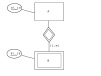
\includegraphics[scale=0.8]{ ./images/5.png }
  \end{center}

  \begin{align*}
    Concave\ Down:\ (-\infty, -1)\cup(1,\infty) \\
    Concave\ Up:\ (-1,1) \\
    Inflection\ Points:\ f(-1) = \frac{1}{4}\\
    f(1) = \frac{1}{4}
  .\end{align*}

  \begin{mdframed}
    \textbf{Example:}
    \begin{align*}
      f(x) = x\sqrt{x+1}
    .\end{align*}
  \end{mdframed}
  \bigbreak \noindent 
  \textit{Rewrite:}
  \begin{align*}
    f(x) = x(x+1)^{\frac{1}{2}}
  .\end{align*}

  \bigbreak \noindent 
  \textit{Find Domain:}
  \begin{align*}
    x+1 \geq 0 \\
    x \geq -1
  .\end{align*}
  \begin{align*}
    D:\ [-1, \infty)
  .\end{align*}

  \bigbreak \noindent 
  \textit{Find $f^{\prime}(x)$:}
  \begin{align*}
    f^{\prime}(x) = (x)[\frac{1}{2}(x+1)^{-\frac{1}{2}}] + (x+1)^{\frac{1}{2}} \\
    = \frac{x}{2(x+1)^{\frac{1}{2}}} + (x+1)^{\frac{1}{2}} \\
    = \frac{x}{2(x+1)^{\frac{1}{2}}} + \frac{2(x+1)^{\frac{1}{2}}(x+1)^{\frac{1}{2}}}{2(x+1)^{\frac{1}{2}}} \\
    = \frac{x}{2(x+1)^{\frac{1}{2}}} + \frac{2(x+1)}{2(x+1)^{\frac{1}{2}}} \\
    = \frac{x}{2(x+1)^{\frac{1}{2}}} + \frac{2x+2}{2(x+1)^{\frac{1}{2}}} \\
    = \frac{3x+2}{2(x+1)^{\frac{1}{2}}} \\
    = \frac{3x+2}{2\sqrt{x+1}} \\
  .\end{align*}

  \bigbreak \noindent 
  \textit{Find critical values:}

  \bigbreak \noindent 
  \textit{$f^{\prime}(x) = 0 $}:
  \begin{align*}
    3x+2 = 0 \\
    \boxed{x = -\frac{2}{3}}
  .\end{align*}
  \bigbreak \noindent 
  \nt{This is within our domain, so therefore we chillin.}

  \bigbreak \noindent \bigbreak \noindent 
  \textit{$f^{\prime}(x)\ DNE $}:
  \begin{align*}
   At\ x= -1 
  .\end{align*}

  \bigbreak \noindent 
  \nt{Since this is an endpoint, it cannot be a local min or max}

  \bigbreak \noindent 
  \textit{Find concave up or down}

  \bigbreak \noindent 
  \begin{center}
    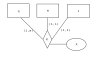
\includegraphics[scale=0.8]{ ./images/6.png }
  \end{center}

  \begin{align*}
    Increasing:\ (-\frac{2}{3}, \infty) \\
    Decreasing:\ (-1, -\frac{2}{3}) \\
    Local\ Min:\ f(-\frac{2}{3}) = -0.4 \\
    Local\ Max:\ None
  .\end{align*}

  \bigbreak \noindent 
  \textit{Find $f^{\prime\prime}(x) $}:
  \begin{align*}
    f^{\prime\prime}(x) = \frac{2(x+1)^{\frac{1}{2}}(3) - (3x+2)(\frac{1}{2})(2)(x+1)^{-\frac{1}{2}}}{[2(x+1)^{\frac{1}{2}}]^{2}} \\
    = \frac{2(x+1)^{\frac{1}{2}}(3) - (3x+2)(x+1)^{-\frac{1}{2}}}{[2(x+1)^{\frac{1}{2}}]^{2}} \\
    = \bigg(\frac{2(x+1)^{\frac{1}{2}}(3) - (3x+2)(\frac{1}{(x+1)^{\frac{1}{2}}})}{4(x+1)}\bigg) \cdot (x+1)^{\frac{1}{2}} \\
    = \frac{6(x+1)-(3x+2)}{4(x+1)^{\frac{3}{2}}} \\
    = \frac{3x+4}{4(x+1)^{\frac{3}{2}}}
  .\end{align*}

  \bigbreak \noindent 
  \textit{Find inflection points:}

  \bigbreak \noindent 
  \textit{$f^{\prime\prime}(x) = 0 $}:
  \begin{align*}
    3x+4 = 0 \\
    x = -\frac{4}{3} \notin D
  .\end{align*}

  \bigbreak \noindent 
  \textit{$f^{\prime\prime}\ DNE $}:
  \begin{align*}
    4(x+1)^{\frac{3}{4}} = 0 \\
    x= -1
  .\end{align*}

  \bigbreak \noindent 
  \nt{Also not a contender because -1 is an endpoint}

  \bigbreak \noindent 
  \textit{Number Line:}

  \bigbreak \noindent 
  \begin{center}
    \includegraphics[scale=1]{ ./images/7.png }
  \end{center}

  \bigbreak \noindent 
  \begin{align*}
    Concave\ Up:\ (-1,\infty) \\
    Concave\ Down:\ None \\
    No\ Inflection\ Points
  .\end{align*}


  \pagebreak \bigbreak \noindent
  \begin{Large}
      \begin{mdframed}
          \begin{center}
              \textbf{4.4}
          \end{center}
      \end{mdframed}
  \end{Large}
  \begin{Large}
      \begin{center}
          \textbf{Indeterminate Form and L'Hospital's Rule}
      \end{center}
  \end{Large}
  \line(1,0){490}
  
  \bigbreak \noindent 
  \begin{mdframed}
    \bigbreak \noindent 
    If:
    \begin{align*}
      \lim_{x \to a}{f(x) = 0}\ and\ \lim_{x \to a}{g(x) = 0} 
    .\end{align*}
    \bigbreak \noindent 
    OR:
    \begin{align*}
      \lim_{x \to a}{f(x)= \pm \infty}\ and\ \lim_{x \to a}{g(x) = \pm \infty}
    .\end{align*}
    \bigbreak \noindent 
    Then:
    \begin{align*}
      \lim_{x \to a}{\frac{f(x)}{g(x)}} = \lim_{x \to a}{\frac{f^{\prime}(x)}{g^{\prime}(x)}}   
    .\end{align*}
    \bigbreak \noindent 
    Provided f and g are differentiable on interval I containing a, $g^{\prime}(x) \neq 0$, the limit on right side exists
  \end{mdframed}
  
  \bigbreak \noindent 
  \nt{To be able to use L'Hospital's rule, we need indeterminate forms of type $\frac{0}{0}\ or\ \frac{\infty}{\infty}$}

  \bigbreak \noindent 
  \begin{mdframed}
    \textbf{Type $0 \cdot \infty $}
    \bigbreak \noindent 
    We need to change to type $\frac{0}{0} or \frac{\infty}{\infty}$
  \end{mdframed}

  \bigbreak \noindent 
  \begin{mdframed}
    \textbf{Example:}
    \begin{align*}
      \lim_{x \to -\infty}{x^{2}e^{x}}
    .\end{align*}
  \end{mdframed}

  \bigbreak \noindent 
  \textit{Since:}
  \begin{align*}
    \lim_{x \to -\infty}{x^{2}} = \infty 
    \lim_{x \to -\infty}{e^{x}} = 0
  .\end{align*}

  \bigbreak \noindent 
  \textit{We have type $\infty \cdot 0 $}, which is an indeterminate form. But we need 
  to change it to one of the two types described above.

  \bigbreak \noindent
  \textit{So:}
  \begin{align*}
    \lim_{x \to -\infty}{\frac{x^{2} \rightarrow \infty}{e^{-x} \rightarrow \infty}}
  \end{align*}

  \bigbreak \noindent 
  \textit{Now we have the form $\frac{\infty}{\infty}$}, so know we can use L'Hospital's Rule.

  \begin{align*}
    L'H = \lim_{x \to -\infty}{\frac{2x \rightarrow -\infty}{-e^{-x} \rightarrow -\infty}}
  .\end{align*}

  \bigbreak \noindent 
  \textit{Now take the derivative again:}
  \begin{align*}
    L'H = \lim_{x \to -\infty}{\frac{2 \rightarrow 2}{e^{-x} \rightarrow \infty}} \\
    \boxed{= 0}
  .\end{align*}

  \bigbreak \noindent 
  \textit{Since we have a constant over infinity, the expression is approaching zero.}

  \bigbreak \noindent 
  \begin{mdframed}
    \textbf{Type $\infty - \infty$}
    \bigbreak \noindent 
    Change this to type $\frac{0}{0}\ or\ \frac{\infty}{\infty}$ by:
    \begin{itemize}
      \item Common denominators
      \item rationalization
      \item factoring
    \end{itemize}
  \end{mdframed}

  \bigbreak \noindent 
  \begin{mdframed}
    \textbf{Example:}
    \begin{align*}
      \lim_{x \to 0+}{\csc{x} - \cot{x}}
    .\end{align*}
  \end{mdframed}

  \begin{align*}
    \lim_{x \to 0+}{\csc{x}} = \infty\ \ \lim_{x \to 0+}{\cot{x}} = \infty
  .\end{align*}

  \bigbreak \noindent 
  \textit{So we have an indeterminate form of the type $\infty -\infty $}, therefore we will rewrite it 
  using the option \textbf{\textit{common denominators}}

  \begin{align*}
    \lim_{x \to 0+}{\frac{1}{\sin{x}} - \frac{\cos{x}}{\sin{x}}} \\
    \lim_{x \to 0+}{\frac{1-\cos{x}}{\sin{x}}}
  .\end{align*}
  \bigbreak \noindent

  \bigbreak \noindent 
  \textit{Now if we plug in zero we get:}
  \begin{align*}
    \frac{0}{0}
  .\end{align*}

  \bigbreak \noindent 
  \textit{Now we can use L'Hospital's Rule}

  \begin{align*}
    L'H = \lim_{x \to 0+}{\frac{\sin{x}}{\cos{x}}}
  .\end{align*}

  \bigbreak \noindent 
  \textit{Now again plug in zero and we get:}
  \begin{align*}
    \frac{0}{1} \\
    \boxed{=0}
  .\end{align*}

  \pagebreak \bigbreak \noindent
  \begin{mdframed}
    \textbf{Types:}
    \begin{itemize}
      \item $0^{0} $
      \item $\infty^{0} $
      \item $1^{\infty}$
    \end{itemize}
    \bigbreak \noindent 
    Change to type $\frac{0}{0}\ or\ \frac{\infty}{\infty}$ by taking ln of the function or writing as an exponential
    \bigbreak \noindent 
    If:
    \begin{align*}
      \lim_{x \to a}{\ln{f(x)} = k}
    .\end{align*}
    \bigbreak \noindent 
    Then:
    \begin{align*}
      \lim_{x \to a}{f(x)} = \lim_{x \to a}{e^{\ln{f(x)}}} \\
      = e^{ \lim_{x \to a}{\ln{f(x)}}} \\
      = e^{k}
    .\end{align*}
  \end{mdframed}

  \bigbreak \noindent 
  \begin{mdframed}
    \textbf{Example: }
    \begin{align*}
      \lim_{x \to \infty}{(e^{x}+x)^{\frac{1}{x}}}
    .\end{align*}
  \end{mdframed}

  \begin{align*}
    \lim_{x \to \infty}{e^{x}} = \infty\ and\ \lim_{x \to \infty}{x} = \infty
  .\end{align*}

  \bigbreak \noindent 
  \textit{So the base is approaching infinity}

  \bigbreak \noindent 
  \textit{And:}
  \begin{align*}
    \lim_{x \to \infty}{\frac{1}{x}} = 0
  .\end{align*}

  \bigbreak \noindent 
  \textit{So we have an indeterminate type of the form:}
  \begin{align*}
    \infty^{0}
  .\end{align*}

  \bigbreak \noindent 
  \textit{So we need to find the limit of the natural log of the function:}

  \begin{align*}
    \lim_{x \to \infty}{\ln{(e^{x}+x)^{\frac{1}{x}}}} \\
    =\lim_{x \to \infty}{\frac{1}{x}\ln{(e^{x}+x)}} \\
    = \lim_{x \to \infty}{\frac{\ln{(e^{x}+x)}}{x}}
  .\end{align*}

  \bigbreak \noindent 
  \textit{since both the numerator and denominator is approaching infinity, we have an indeterminate form of the type $\frac{\infty}{\infty} $}, so we can use L'Hospital's Rule

  \begin{align*}
    L'H = \lim_{x \to \infty}{\frac{\frac{1}{e^{x}+x}(e^{x}+1)}{1}} \\
    = \lim_{x \to \infty}\frac{e^{x}+1}{e^{x}+x}
  .\end{align*}

  \bigbreak \noindent 
  \textit{Still, we have the indeterminate form of the type $\frac{in}{in} $}, so we
  must once again use L'Hospital's Rule

  \begin{align*}
    L'H = \lim_{x \to \infty}{\frac{e^{x}}{e^{x}+1}}
  .\end{align*}

  \bigbreak \noindent 
  \textit{Still, we have the indeterminate form of the type $\frac{in}{in} $}, so we
  must once again use L'Hospital's Rule

  \begin{align*}
    L'H = \lim_{x \to \infty}{\frac{e^{x}}{e^{x}}} \\
    = \lim_{x \to \infty}{1} \\ =1
  .\end{align*}

  \bigbreak \noindent
  \textit{Therefor:}
  \begin{align*}
   \lim_{x \to \infty}{(e^{x}+x)^{\frac{1}{x}}} = e^{1} \\
   = e
  \end{align*}

  \bigbreak \noindent 
  \begin{mdframed}
    \textbf{Example:}
    \begin{align*}
      \lim_{x \to 1}{\frac{1-x+\ln{x}}{1+\cos{9\pi x}}}
    .\end{align*}
  \end{mdframed}

  \begin{align*}
    \lim_{x \to 1}{1-x+\ln{x}} = 0
  .\end{align*}
  \begin{align*}
    \lim_{x \to 1}{1+\cos{9\pi x}} = 0
  .\end{align*}

  \bigbreak \noindent 
  \textit{So we have an indeterminate form of the type $\frac{0}{0} $}, so we can use L'Hospital's Rule

  \begin{align*}
    L'H = \lim_{x \to 1}{\frac{-1+\ln{x}}{-\sin{(9\pi x) \cdot 9\pi}}}
  .\end{align*}

  \bigbreak \noindent 
  \textit{Still have $\frac{0}{0}$}

  \begin{align*}
    L'H = \lim_{x \to 1}{\frac{-\frac{1}{x^{2}}}{-\cos{9\pi x}(81 \pi^{2})}} \\
    = \boxed{-\frac{1}{81\pi^{2}}}
  .\end{align*}

  \pagebreak \bigbreak \noindent
  \bigbreak \noindent
  \begin{mdframed}
  \begin{large}
      \begin{center}
          \textbf{Graphs to Review for 4.4}
      \end{center}
  \end{large}
  \end{mdframed}
  \line(1,0){490}
  \bigbreak \noindent \bigbreak
  \begin{mdframed}
    \textbf{$e^{x}\ and\ e^{-x}:$}
    \bigbreak \noindent 
    \begin{center}
      \includegraphics[scale=0.5]{ ./images/8.png }
    \end{center}
  \end{mdframed}

  \bigbreak \noindent 
  \begin{mdframed}
    \textbf{Graph of Sin and Csc:}
    \bigbreak \noindent 
    \begin{center}
      \includegraphics[scale=.5]{ ./images/9.png }
    \end{center}
    \bigbreak \noindent 
    Asymptotes at: $-2\pi, -\pi, \pi, 2\pi $
  \end{mdframed}

  \pagebreak \bigbreak \noindent
  \begin{mdframed}
    \textbf{Graph of Cos and Sec:} 
    \bigbreak \noindent 
    \begin{center}
      \includegraphics[scale=0.5]{ ./images/10.png}
    \end{center}
    \bigbreak \noindent 
    Asymptotes at: $\frac{\pi}{2}, \frac{3\pi}{2} $
  \end{mdframed}

  \bigbreak \noindent 
  \begin{mdframed}
    \textbf{Graph of tan and cot:}
    \bigbreak \noindent 
    \begin{center}
      \includegraphics[scale=0.5]{ ./images/11.png }
    \end{center}
    \bigbreak \noindent 
    \begin{center}
      \includegraphics[scale=0.6]{ ./images/12.png }
    \end{center}
  \end{mdframed}

  \pagebreak \bigbreak \noindent
  \begin{mdframed}
    \begin{center}
      \includegraphics[scale=.95]{ ./images/13.png }
    \end{center}
  \end{mdframed}

  \pagebreak \bigbreak \noindent
  \begin{Large}
      \begin{mdframed}
          \begin{center}
              \textbf{4.5}
          \end{center}
      \end{mdframed}
  \end{Large}
  \begin{Large}
      \begin{center}
          \textbf{Summary of Curve Sketching}
      \end{center}
  \end{Large}
  \line(1,0){490}

  \bigbreak \noindent 
  \begin{mdframed}
    \textbf{Example:}
    \begin{align*}
      y = x^{4} + 4x^{3}
    .\end{align*}
    \bigbreak \noindent 
    Use the guidelines of this section to sketch the curve.
  \end{mdframed}

  \bigbreak \noindent 
  \textbf{\textit{\underline{A: Domain: Since this is a polynomial (binomial), the domain is $ \mathbb{R} $ }}}

  \bigbreak \noindent 
  \textbf{\textit{\underline{B: Intercepts}}}

  \bigbreak \noindent 
  \textit{x intercepts:}
  \begin{align*}
    0 = x^{4} + 4x^{3}  \\
    0 = x^{3}(x+4) \\
  .\end{align*}
  \begin{align*}
    x^{3} = 0 \\
    x = 0
  .\end{align*}
  \begin{align*}
    x+4 = 0 \\
    x = -4
  .\end{align*}

  \bigbreak \noindent 
  \textit{Therefore the x-ints are:}
  \begin{align*}
    \boxed{(0,0)\ and\ (-4,0)}
  .\end{align*}

  \bigbreak \noindent 
  \textit{y intercepts:}
  \begin{align*}
    y(0) (0)^{4} + 4(0)^{3} \\
    \boxed{= 0}
  .\end{align*}

  \bigbreak \noindent 
  \textbf{\textit{\underline{C: Symmetry: Odd/Even/Neither}}}
  \begin{itemize}
    \item Even $\longrightarrow$ symmetric with resepect to y-axis
      \begin{itemize}
        \item $f(-x) = f(x) $
      \end{itemize}
    \item Odd $\longrightarrow$ symmetric with resepect to the orgin
      \begin{itemize}
        \item $f(-x) = -f(x) $
      \end{itemize}
  \end{itemize}

  \bigbreak \noindent 
  \textit{Check if even:}
  \begin{align*}
    f(x) = x^{4} + 4x^{3} \\
    f(-x) = (-x)^{4} + 4(-x)^{3} \\
    = x^{4} -4x^{3} \\
    \boxed{Not\ Even}
  .\end{align*}

  \bigbreak \noindent 
  \textit{Check if odd:}
  \begin{align*}
    f(x) = x^{4} + 4x^{3} \\
    f(-x) = (-x)^{4} + 4(-x)^{3} \\
    = x^{4} -4x^{3} \\
    \boxed{Not\ Odd}
  .\end{align*}

  \bigbreak \noindent 
  \textbf{\textit{\underline{Therefore:}}}
  \begin{center}
    \textbf{C: Neither}
  \end{center}

  \bigbreak \noindent  \bigbreak \noindent 
  \textbf{\textit{\underline{D: Asymptotes}}}

  \bigbreak \noindent 
  \textit{Recall:}
  \begin{center}
    \textbf{Horizontal Asymptotes:}
  \end{center}
  \begin{align*}
    \lim_{x \to \infty}{f(x) = ?} \\
    \lim_{x \to -\infty}{f(x) = ?}
  .\end{align*}

  \bigbreak \noindent
  \textit{So:}
  \begin{align*}
    \boxed{\lim_{x \to \infty}{(x^{4}+4x^{3})} = \infty}
  \end{align*}

  \bigbreak \noindent 
  \textit{And:}
  \begin{align*}
    \lim_{x \to -\infty}{(x^{4}+4x^{3})} = \infty - \infty
  .\end{align*}

  \bigbreak \noindent 
  \textit{Since we have an indeterminate form of the type $\infty -\infty$}, we can work
  around this by factoring

  \begin{align*}
    \lim_{x \to -\infty}{x^{4}(1+\frac{4}{x})} \\
    \infty(1+0) = \infty
  .\end{align*}

  \bigbreak \noindent 
  \textit{Therefore:}
  \begin{align*}
    \boxed{\lim_{x \to -\infty}{x^{4}+4x^{3}} = \infty}
  .\end{align*}

  \bigbreak \noindent 
  \textit{Since these limits dont equal a constant, we have no Horizontal Asymptote}

  \bigbreak \noindent 
  \textit{Recall:}
  \begin{center}
    \textbf{Vertical Asymptotes:}
  \end{center}
  \bigbreak \noindent 
  \textit{recall that vertical Asymptotes only apply to rational functions, to find the vertical Asymptote, first get the function
    to simpliest form and find where the function cannot equal 0, ie set the denominator equal to zero.
  }

  \bigbreak \noindent 
  \textit{Recall:}
  \begin{center}
    \textbf{Oblique (Slant) Asymptote:}
  \end{center}
  \bigbreak \noindent 
  \textit{For a rational function whose numerator's defree is 1 more than its denominator's degree. After
    long division, the quotient is the equation of the Oblique Asymptote.
  }
  \bigbreak \noindent 
  \textit{Example:}
  \begin{align*}
    f(x) = \frac{2x^{3} + x^{2} + x +3}{x^{2} + 2x}
  .\end{align*}

  \bigbreak \noindent 
  \textit{Long division:}
  \begin{align*}
    x^{2}+2x \overline{)2x^{3}+x^{2}+x+3}
  .\end{align*}
  \bigbreak \noindent 
  \begin{align*}
    o.a\:\ y= 2x-3
  .\end{align*}
  \bigbreak \noindent 
  \nt{Remainder is not included}
  \bigbreak \noindent 
  \textbf{\textit{\underline{Therefore:}}}
  \begin{center}
    \textbf{D: No Horizontal/Vertical or Oblique Asymptotes}
  \end{center}

  \bigbreak \noindent \bigbreak \noindent 
  \textbf{\textit{\underline{E: Intervals of Increase/Decrease}}}
  \begin{align*}
    f(x) = x^{4} + 4x^{3}
  .\end{align*}

  \bigbreak \noindent 
  \textit{Find $f^{\prime}(x)$}:
  \begin{align*}
    f^{\prime}(x) = 4x^{3} + 12x^{2}
  .\end{align*}

  \bigbreak \noindent 
  \textit{Critical values}
  \begin{align*}
    4x^{3} + 12x^{2} = 0 \\ 
    4x^{2}(x + 3) = 0 \\
  .\end{align*}
  \begin{align*}
    4x^{2} = 0 \\
    \boxed{x = 0}
  .\end{align*}
  \begin{align*}
    x+ 3 = 0  \\
    \boxed{x = -3}
  .\end{align*}
  
  \bigbreak \noindent 
  \textit{Make number line and test points with $f^{\prime}(x)$}:

  \bigbreak \noindent 
  \begin{center}
    \includegraphics[scale=0.7]{ ./images/14.png}
  \end{center}

  \bigbreak \noindent 
  \textbf{\textit{\underline{E:}}}
  \begin{align*}
    Increasing:\ (-3,0) \cup (0,\infty)\\
    Derceasing:\ (-\infty, -3)
  .\end{align*}

  \pagebreak \bigbreak \noindent
  \textbf{\textit{\underline{F: Local Minimum/Maximum}}}

  \bigbreak \noindent 
  \textit{Local Min: Since $f^{\prime}(x)$} switches from negative to positive at -3, we have a local min at f(-3)
  \begin{align*}
    f(-3) = (-3)^{4} + 4(-3)^{3} \\
    \boxed{=-27}
  .\end{align*}

  \bigbreak \noindent 
  \textit{Local Max: Since $f^{\prime}(x)$} has not switch from positive to negative, we have no local max.

  \bigbreak \noindent 
  \textbf{\textit{\underline{Therefore:}}}
  \begin{align*}
    Local\ Min:\ f(-3) = -27 \\
    Local\ Max:\ None
  .\end{align*}

  \bigbreak \noindent 
  \textbf{\textit{\underline{G: Concavity and Inflection Points:}}}

  \bigbreak \noindent 
  \textit{Recall:}
  \begin{align*}
    f^{\prime}(x) = 4x^{3}+12x^{2}
  .\end{align*} 

  \bigbreak \noindent 
  \textit{$f^{\prime\prime}(x)$}:
  \begin{align*}
    f^{\prime\prime}(x) = 12x^{2} + 24x
  .\end{align*}

  \bigbreak \noindent 
  \textit{Find possible inflection points:}
  \begin{align*}
    12x^{2} +24x = 0 \\
    12x(x+2) = 0 \\
    12x = 0 \\
    \boxed{x= 0} \\
    x+2 = 0 \\
    \boxed{x= -2}
  .\end{align*}

  \bigbreak \noindent 
  \textit{Make number line to test intervals of concavity:}

  \bigbreak \noindent 
  \begin{center}
    \includegraphics[scale=0.7]{ ./images/15.png }
  \end{center}

  \bigbreak \noindent 
  \textbf{\textit{\underline{G: Therefore}}}
  \begin{align*}
    Concave\ up:\ (-\infty, -2) \cup (0,\infty) \\
    Concave\ Down:\ (-2,0) \\
    Inflection\ Points:\ f(-2) = (-2)^{4} + 4(-2)^{3} \\
    \boxed{= -16} \\
    \boxed{f(0) = 0}
  .\end{align*}

  \pagebreak \bigbreak \noindent
  \textbf{\textit{\underline{H: Sketch the Curve:}}}

  \bigbreak \noindent 
  \textit{List all information:}
  \begin{align*}
    Int:\ (0,0),\ (-4,0) \\
    Local\ Min:\ f(-3) = -27 \\
    Inflection\ Points:\ f(-2) = -16\ and\ f(0) = 0
  .\end{align*}

  \bigbreak \noindent 
  \textit{Sketch Graph:}

  \bigbreak \noindent 
  \begin{center}
    \includegraphics[scale=0.7]{ ./images/17.png }
  \end{center}

  \bigbreak \noindent 
  \begin{mdframed}
    \textbf{Example:}
    \begin{align*}
      y= \frac{1}{x^{2}-16}
    .\end{align*}
  \end{mdframed}

  \bigbreak \noindent 
  \textbf{\textit{\underline{A: Domain}}}
  \begin{align*}
    x^{2} - 16 \neq 0 \\
    x^{2} \neq 16 \\
    x \neq \pm 4 \\
    \boxed{(-\infty, -4) \cup (-4,4) \cup (4,\infty)}
  .\end{align*}

  \bigbreak \noindent 
  \textbf{\textit{\underline{B: Intercepts:}}}
  \bigbreak \noindent 
  \textit{x-int}
  \begin{align*}
   0 = \frac{1}{x^{2}-16} \\
   1= 0 \\
   \boxed{\text{No x intercept}}
  .\end{align*}

  \bigbreak \noindent 
  \textit{y-int}
  \begin{align*}
    y(0) = \frac{1}{(0)^{2}-16} \\
    = -\frac{1}{16} \\
    \boxed{\bigg(0, -\frac{1}{16}\bigg)}
  .\end{align*}

  \bigbreak \noindent 
  \textbf{\textit{\underline{C: Asymptotes:}}}

  \bigbreak \noindent 
  \textit{Horizontal Asymptotes:}
  \begin{align*}
    \lim_{x \to \infty}{\frac{1}{x^{2}-16}} = 0 \\
    and\\
    \lim_{x \to -\infty}{\frac{1}{x^{2}-16}} = 0
  .\end{align*}
  \begin{align*}
    H.A:\ y=0
  .\end{align*}

  \bigbreak \noindent 
  \nt{Another way to check: if you have a rational function is the degree of the numerator is either equal to the 
    degree of the denominator, or lower
  }

  \bigbreak \noindent 
  \textit{Vertical Asymptotes: (When the denominator equals 0, and is in simpliest form)}
  \begin{align*}
    \boxed{V.A:\ x=4,x=-4}  
  .\end{align*}

  \bigbreak \noindent 
  \textit{Slant Asymptote:}
  \begin{align*}
    \boxed{\text{No slant asymptote}}
  .\end{align*}
  \bigbreak \noindent 
  \nt{You cannot have both a Horizontal and slant asymptote, since we know there is a Horizontal asymptote, therefore cannot have a slant}

  \bigbreak \noindent 
  \textbf{\textit{\underline{D: symmetric}}}

  \bigbreak \noindent 
  \textit{Even:}
  \begin{align*}
    f(-x) = \frac{1}{(-x)^{2}-16} \\
    =\frac{1}{x^{2}-16}
  .\end{align*}

  \bigbreak \noindent 
  \textit{Since $f(-x)=f(x)$}, the function is symmetric about the y axis.

  \bigbreak \noindent 
  \textbf{\textit{\underline{E: increasing/decreasing}}}
  \begin{align*}
    y^{\prime} = (x^{2}-16)^{-1} \\
    -1(x^{2}-16)^{-2}(2x) \\
    \frac{-2x}{(x^{2}-16)^{2}}
  .\end{align*}

  \bigbreak \noindent 
  \textit{$f^{\prime}(x) = 0$}
  \begin{align*}
    -2x = 0 \\
    \boxed{x = 0}
  .\end{align*}

  \bigbreak \noindent 
  \textit{$f^{\prime}(x)$} DNE
  \begin{align*}
    (x^{2}-16)^{2} = 0  \\
    x^{2}- 16 = 0 \\
    x^{2} = 16 \\
    \boxed{x = \pm 4 \notin D}
  .\end{align*}

  \bigbreak \noindent 
  \nt{They are not local min/max, or critical values, but we will still list them on our number line}

  \bigbreak \noindent 
  \begin{center}
    \includegraphics[scale=0.7]{ ./images/18.png }
  \end{center}
  \begin{align*}
    Increasing:\ (-\infty, -4) \cup (-4,0) \\
    Derceasing:\ (0,4) \cup (4,\infty)
  .\end{align*}

  \bigbreak \noindent 
  \textbf{\textit{\underline{F: Local Min/Max}}}
  \bigbreak \noindent 
  \textit{Local Max: goes from positive to negative at 0}
  \begin{align*}
    \boxed{f(0) = -\frac{1}{16}}
  .\end{align*}
  \bigbreak \noindent 
  \textit{local min: doesn't go from negative to positive so:}
  \begin{align*}
    \boxed{\text{No local min}}
  .\end{align*}

  \bigbreak \noindent 
  \textbf{\textit{\underline{G: Concavity, Inflection Points:}}}

  \bigbreak \noindent 
  \textit{If:}
  \begin{align*}
    y^{\prime} = \frac{-2x}{(x^{2}-16)^{2}}
  .\end{align*}
  
  \bigbreak \noindent 
  \textit{$y^{\prime\prime}$}:
  \begin{align*}
    y^{\prime\prime} = \frac{-2(x^{2}-16)^{2}+8x^{2}(x^{2}-16)}{(x^{2}-16)^{4}} \\
    = \frac{2(x^{2}-16)[-(x^{2}-16)+4x^{2}]}{(x^{2}-16)^{4}} \\
    = \frac{2[-(x^{2}-16)+4x^{2}]}{(x^{2}-16)^{3}}  \\
    = \frac{2[-x^{2}+16+4x^{2}]}{(x^{2}-16)^{3}}  \\
    = \frac{2(3x^{2}+16)}{(x^{2}-16)^{3}}  \\
  .\end{align*}

  \bigbreak \noindent 
  \textit{$y^{\prime\prime} = 0$}:
  \begin{align*}
   2(3x^{2}+16) =0 \\
   3x^{2} = -16 \\
   x^{2} = -8 \\
   \boxed{None}
  .\end{align*}

  \bigbreak \noindent 
  \textit{$y^{\prime\prime} = $} DNE:
  \begin{align*}
    x^{2}-16 = 0 \\
    x = \pm 4 \notin d
  .\end{align*}

  \bigbreak \noindent 
  \nt{They wont be inflection points, but still need to list them when testing for concavity.}

  \bigbreak \noindent 
  \begin{center}
    \includegraphics[scale=0.7]{ ./images/19.png }
  \end{center}
  \begin{align*}
    Concave:\ Up\ (-\infty, -4) \cup (4,\infty) \\
    Concave:\ Down\ (-4,4) \\
    None
  .\end{align*}

  \pagebreak \bigbreak \noindent
  \textbf{\textit{\underline{H: Sketch Graph}}}

  \bigbreak \noindent 
  \textit{List values:}
  \begin{align*}
    y-int:\ (0, \frac{-1}{16}) \\
    V.A:\ x=\pm 4 \\
    H.A:\ y = 0 \\
    y-axis\ symmetry
  .\end{align*}

  \bigbreak \noindent 
  \begin{center}
    \includegraphics[scale=0.7]{ ./images/20.png }
  \end{center}

  \pagebreak \bigbreak \noindent
  \begin{Large}
      \begin{mdframed}
          \begin{center}
              \textbf{4.7}
          \end{center}
      \end{mdframed}
  \end{Large}
  \begin{Large}
      \begin{center}
          \textbf{Optimization Problems:}
      \end{center}
  \end{Large}
  \line(1,0){490}
  
  \bigbreak \noindent 
  \begin{mdframed}
    \textbf{Strategy:}
    \begin{enumerate}
      \item Read the problem carefully
      \item Draw a diagram whenever possible 
      \item Introducte notation
      \item Expess the quantity to be optimized in terms of other variables.
      \item Reduce the number of variables from Step 4 to only 1 (write a function of 1 variable)
      \item find the absolute minimum/maximum
    \end{enumerate}
  \end{mdframed}

  \bigbreak \noindent 
  \begin{mdframed}
    \textbf{Example: Find two numbers whose difference is 100 and whose product is a minimum}
  \end{mdframed}

  \bigbreak \noindent
  \textit{So let the two numbers be x and y}
  \begin{align*}
    x-y=100
  .\end{align*}
  
  \bigbreak \noindent 
  \textit{And let product $p$, be:}
  \begin{align*}
    p = xy
  .\end{align*}

  \bigbreak \noindent 
  \textit{Solve for x:}
  \begin{align*}
    x = y+100
  .\end{align*}

  \bigbreak \noindent 
  \textit{Now:}
  \begin{align*}
    p(y) = (y+100)y \\
    p(y) = y^{2} + 100y
  .\end{align*}

  \bigbreak \noindent 
  \textit{Now we can take the derivitative}
  \begin{align*}
    p^{\prime}(y) =2y+100
  .\end{align*}

  \bigbreak \noindent 
  \textbf{\textit{\underline{find critical values:}}}
  
  \bigbreak \noindent 
  \textit{$p^{\prime}(y)=  0$}:
  \begin{align*}
    2y+100 = 0 \\
    y=  -50
  .\end{align*}

  \bigbreak \noindent 
  \textit{$p^{\prime}(y)$} = DNE
  \begin{center}
    none
  \end{center}

  \pagebreak \bigbreak \noindent
  \textit{Check if y = -50 yields a minimum, by applying the second derivative test:}
  \begin{align*}
    y^{\prime\prime} = 2
  .\end{align*}
  \textit{since $2>0 $, $p$ is concave up and -50 is indeed a min}

  \bigbreak \noindent
  \textit{Find x (second number)}:

  \begin{align*}
    x = -50 + 100    
  .\end{align*}

  \bigbreak \noindent 
  \textbf{\textit{\underline{Therefore:}}}

  \bigbreak \noindent 
  \textit{The two numbers are 50 and -50}

 \bigbreak \noindent 
 \begin{mdframed}
   \textbf{Example: A rectangular storage container with an open top is to have a volume of $10m^{3}$. The length of its base is twice the width. Material for the base costs \$10 per square meter. Material 
     for the sides costs \$6 per square meter. Find the cost of materials for the cheapest such container.
   }
 \end{mdframed} 
 
 \bigbreak \noindent 
 \textit{So:}
 \bigbreak \noindent 
 \begin{center}
   \textbf{Minimize Cost!}
 \end{center}
 \begin{center}
   \includegraphics[scale=0.5]{ ./images/21.png  }
 \end{center}
 \bigbreak \noindent 
 \textit{And we know:}
 \begin{align*}
   V = 10m^{3}
 .\end{align*}

 \bigbreak \noindent 
 \textit{Function for cost of base:}
 \begin{align*}
   C = (2x)(x)(10) + (h)(x)(6)(2) + (h)(2x)(6)(2)
 .\end{align*}

 \bigbreak \noindent \begin{center}
   \includegraphics[scale=.5]{ ./images/22.png }
 \end{center}

 \bigbreak \noindent 
 \textit{Cleanup:} 
 \begin{align*}
   C = 20x^{2} + 12xh + 24xh \\
   C = 20x^{2} + 36xh
 .\end{align*}

 \bigbreak \noindent 
 \textit{Eliminate one of the variables:}
 \bigbreak \noindent 
 \textit{If:}
 \begin{align*}
   v=10m^{3} \\
   and\\
   v = b \cdot w \cdot h
 .\end{align*}
 \bigbreak \noindent 
 \textit{Then:}
 \begin{align*}
   10 = (2x)(x)(h) \\
   10 = 2x^{2}h \\
   5 = x^{2}h \\
   h = \frac{5}{x^{2}}
 .\end{align*}

 \bigbreak \noindent 
 \textit{Now that we have h, we will substitute it in c(x)}
 \begin{align*}
   c(x) = 20x^{2}+36x(\frac{5}{x^{2}}) \\
   c(x) = 20x^{2} + \frac{180}{x}
 .\end{align*}

 \bigbreak \noindent 
 \textit{Compute $c^{\prime}(x)$}
 \begin{align*}
   c^{\prime}(x) = 40x - \frac{180}{x^{2}} \\
   = \frac{40x^{3}-180}{x^{2}}
 .\end{align*}

 \bigbreak \noindent 
 \textit{Find critical values:}

 \begin{align*}
   40x^{3} -180 = 0  \\
   40x^{3} = 180 \\
   x^{3} = \frac{9}{2} \\
   x = \sqrt[3]{\frac{9}{2}}
 .\end{align*}

 \bigbreak \noindent 
 \textit{$c^{\prime}(x) =\ DNE $}
 \begin{align*}
   x = 0 \notin d
 .\end{align*}
 \bigbreak \noindent 
 \nt{not in domain because for x to be zero we would have no box at all.}

 \bigbreak \noindent 
 \textit{confirm that this is a minimum by applying the second derivitative test.}

 \begin{align*}
   c^{\prime\prime}(x) = 40 +\frac{360}{x^{3}}
 .\end{align*}
 \begin{align*}
   c(\sqrt[3]{\frac{9}{2}}) = 40 + \frac{360}{\frac{9}{2}} > 0
 .\end{align*}

 \bigbreak \noindent 
 \textit{Since we now know that it is concave up, it does indeed yield a min.}
 
 \bigbreak \noindent 
 \textit{Now substitute the critical value into the cost function:}
 \begin{align*}
   c(\sqrt[3]{\frac{9}{2}}) = 20(\sqrt[3]{\frac{9}{2}})^{2} + \frac{180}{\sqrt[3]{\frac{9}{2}}} \\
   \boxed{\approx \$163.54}
 .\end{align*}

 \bigbreak \noindent 
 \begin{mdframed}
   \textbf{Example: Find the point on the line $6x+y=9$ that is closest to the point (-3,1)}
 \end{mdframed}

 \bigbreak \noindent
 \textit{So:}
 \bigbreak \noindent 
 \begin{center}
   \includegraphics[scale=0.8]{ ./images/23.png }
 \end{center}

 \bigbreak \noindent 
 \textit{Goal: minimize distance from (-3,1) to the line}

 \bigbreak \noindent 
 \textit{Recall: Distance formula:}
 \begin{align*}
   d = \sqrt{(x_2 -x_1)^{2}+(y_2-y_1)^{2}}
 .\end{align*}

 \bigbreak \noindent 
 \textit{We will use the point (x, $-6x+9 $)}
 \begin{align*}
   d =\sqrt{(x+3)^{2} + (-6x+9-1)^{2}} \\
   = \sqrt{x^{2}+6x+9 +36x^{2}-96x+64} \\
   = \sqrt{37x^{2}-90x + 73}
 .\end{align*}
 \bigbreak \noindent 
 \textit{This is the function we will differentiate.}

 \bigbreak \noindent 
 \textit{Let D = $d^{2} = 37x^{2}-90x+73$}

 \bigbreak \noindent 
  \nt{Whatever x-value minimizes d also minimizes $D=d^{2}$, which is an easier function to work with}

  \bigbreak \noindent
  \textit{So:}
  \begin{align*}
    D(x) = 37x^{2}-90x+73    
  \end{align*}
  \begin{align*}
    D^{\prime}(x) = 74x - 90
  .\end{align*}

  \bigbreak \noindent 
  \textit{Find critical values:}

  \begin{align*}
    74x-90 = 0 \\
    74x = 90 \\
    x = \frac{90}{74} \\
    x= \frac{45}{37}
  .\end{align*}

  \bigbreak \noindent 
  \textit{confirm that this yeilds a min by using the second deriviative test:}

  \begin{align*}
    D^{\prime\prime}(x) = 74 > 0 
  .\end{align*}

  \bigbreak \noindent 
  \textit{Therefore this does yeild a min}

  \begin{align*}
    y = -6(\frac{45}{37}) + 9 \\
    = \frac{63}{37}
  .\end{align*}

  \bigbreak \noindent 
  \textit{Point:}
  \begin{align*}
    \bigg(\frac{45}{37}, \frac{63}{37}\bigg)
  .\end{align*}

  \pagebreak \bigbreak \noindent
  \begin{Large}
      \begin{mdframed}
          \begin{center}
              \textbf{4.8}
          \end{center}
      \end{mdframed}
  \end{Large}
  \begin{Large}
      \begin{center}
          \textbf{Newton's Method}
      \end{center}
  \end{Large}
  \line(1,0){490}
  
  \bigbreak \noindent \bigbreak \noindent \bigbreak \noindent 
  This method helps us find approximate roots of an equation, which would be impossible to find otherwise.

  \bigbreak \noindent 
  \begin{center}
    \includegraphics[scale=0.3]{ ./images/24.png }
  \end{center}

  \bigbreak \noindent 
  We start first with an approximation $x$, near $r$

  \bigbreak \noindent 
  To find a formula for $x_2$, which lies on the tangent line $L $, we use the point $(x_1,f(x_1))$ and $m=f^{\prime}(x_1) $
  \begin{align*}
    y -y_1 = m(x-x_1) \\
    y - f(x_1) = f^{\prime}(x_1)(x-x_1)
  .\end{align*}

  \bigbreak \noindent 
  Since the second point is $(x_2, 0)$, we have:
  \begin{align*}
    0 - f(x_1) = f^{\prime}(x_1)(x_2-x_1) \\
     = x_2-x_1 \\
    x_2 = x_1 -\frac{f(x_1)}{f^{\prime}(x_1)}
  .\end{align*}

  \bigbreak \noindent \bigbreak \noindent 
  Similalarly, $x_3$:
  \begin{align*}
    x_2 - \frac{f(x_2)}{f^{\prime}(x_2)}
  .\end{align*}

  \bigbreak \noindent \bigbreak \noindent 
  And $x_{n+1}$:
  \begin{align*}
    x_n - \frac{f(x_n)}{f^{\prime}(x_n)}
  .\end{align*}

  \pagebreak \bigbreak \noindent
  \begin{mdframed}
    \textbf{Example: Use Newton's Method with $x_1 = -3$ to find $x_3 $}
    \begin{align*}
      \frac{1}{3}x^{3}+\frac{1}{2}x^{2}+3 = 0
    .\end{align*}
  \end{mdframed} 

  \bigbreak \noindent
  \textit{So:}
  \begin{align*}
    f(x) =\frac{1}{3}x^{3} + \frac{1}{2}x^{2} + 3
  \end{align*}

  \bigbreak \noindent 
  \textit{and $f^{\prime}(x)$}:
  \begin{align*}
    f^{\prime}(x) = x^{2} + x
  .\end{align*}

  \bigbreak \noindent  \bigbreak \noindent 
  \textit{We have $x_1$, so we need to find $x_2$ and $x_3$, ie 2 iterations of Newton's Method}

  \bigbreak \noindent
  \textit{So:}
  \begin{align*}
    x_2 = x_1 - \frac{f(x_1)}{f^{\prime}(x_1)}
  \end{align*}

  \bigbreak \noindent 
  \textit{Which means:}
  \begin{align*}
    x_2 = -3 - \frac{f(-3)}{f^{\prime}(-3)} \\
    = -3 \frac{\frac{1}{3}(-27)+\frac{1}{2}(9)+3}{9-3} \\
    = -3 - \frac{-9 + \frac{9}{2}+3}{6} \\
    = -2.75
  .\end{align*}

  \bigbreak \noindent 
  \textit{Now $x_3 $}:
  \begin{align*}
    x_3 = x_2 - \frac{f(x_2)}{f^{\prime}(x_2)}
  .\end{align*}

  \bigbreak \noindent 
  \textit{which means:}
  \begin{align*}
    x_3 = -2.75 - \frac{f(-2.75)}{f^{\prime}(-2.75)} \\
    \approx -2.7186
  .\end{align*}

  \pagebreak \bigbreak \noindent
  \begin{mdframed}
    \textbf{Example: Use Newton's Method to find all solutions of the equation correct to six decimal places.}
    \begin{align*}
      e^{x} = 3 - 2x 
    .\end{align*}
  \end{mdframed}

  \bigbreak \noindent 
  \begin{center}
    \includegraphics[scale=0.6]{ ./images/25.png }
  \end{center}
  
  \bigbreak \noindent
  \textit{So:}
  \begin{align*}
    f(x) = e^{x} +2x-3
  \end{align*}

  \bigbreak \noindent 
  \textit{$f^{\prime}(x)$}:
  \begin{align*}
    e^{x}+2
  .\end{align*}

  \bigbreak \noindent 
  \textit{to get $x_1$, pick a point from the graph}
  \begin{align*}
    x_1 = 1
  .\end{align*}

  \bigbreak \noindent 
  \textit{Now use Newton's Method}
  \begin{align*}
    x_2 = x_1 - \frac{f(x_1)}{f^{\prime}(x_1)}
  .\end{align*}

  \bigbreak \noindent 
  \textit{Which means:}
  \begin{align*}
    x_2 = 1 - \frac{f(1)}{f^{\prime}(1)} \
    \approx 0.6358
  .\end{align*}

  \bigbreak \noindent 
  \textit{Keep going on calc until answer stops changing}

  \begin{align*}
    x_5 \approx 0.5942049585
  .\end{align*}

  \pagebreak \bigbreak \noindent
  \begin{Large}
      \begin{mdframed}
          \begin{center}
              \textbf{4.9}
          \end{center}
      \end{mdframed}
  \end{Large}
  \begin{Large}
      \begin{center}
          \textbf{Antiderivatives}
      \end{center}
  \end{Large}
  \line(1,0){490}
  

  \bigbreak \noindent \bigbreak \noindent \bigbreak \noindent 
  In this section we'll learn how we can find an unknown function if we know its derivative.  \\
  Let the known derivative be f(x), the unknown function is F(x). \\
  If $F^{\prime}(x)= f(x)$, then F(x) is called the Antiderivative of f(x)

  \bigbreak \noindent 
  \begin{mdframed}
    \textbf{Example: Find F(x) if $f(x) = x^{3} $ and $F^{\prime}(x) =f(x)$}
  \end{mdframed}

  \bigbreak \noindent
  \textit{So:}
  \begin{align*}
    F(x) = \frac{1}{4}x^{4}
  \end{align*}

  \bigbreak \noindent 
  \textit{Check:}
  \begin{align*}
    F^{\prime}(x) = x^{3}
  .\end{align*}

  \bigbreak \noindent \bigbreak \noindent 
  The most general Antiderivative of $f$ on interval $I$ is:
  \begin{align*}
    F(x) + C 
  .\end{align*}

  \bigbreak \noindent \bigbreak \noindent 
  \textit{Since the function could have any contstant attached to it and still yield the same derivitave, we add +C}

  \bigbreak \noindent 
  \begin{center}
    \includegraphics[scale=0.6]{ ./images/26.png }
  \end{center}

  \pagebreak \bigbreak \noindent
  \begin{mdframed}
    \textbf{Example: Find the most general Antiderivative of f(x)}
    \begin{align*}
      f(x) = 8x^{9}-3x^{6}=12x^{3}
    .\end{align*}
  \end{mdframed}

  \bigbreak \noindent
  \textit{So:}
  \begin{align*}
    F(x) = \frac{8x^{9+1}}{9+1} - \frac{3x^{6+1}}{6+1} +\frac{12x^{3+1}}{3+1} + C \\
    = \frac{8x^{10}}{10} -\frac{3x^{7}}{7} +\frac{12x^{4}}{4} + C \\
    = \frac{4}{5}x^{10} - \frac{3}{7}x^{7}+3x^{4} +C
  \end{align*}

  \bigbreak \noindent 
  \begin{mdframed}
    \textbf{Example: }
    \begin{align*}
      f(x) = \frac{5 - 4x^{3} +2x^{6}}{x^{6}}
    .\end{align*}
  \end{mdframed}

  \bigbreak \noindent 
  \textit{Rewrite:}
  \begin{align*}
    f(x) = \frac{5}{x^{6}} -\frac{4x^{3}}{x^{6}} +\frac{2x^{6}}{x^{6}} \\
    = 5x^{-6}-4x^{-3}+2
  .\end{align*}

  \bigbreak \noindent
  \textit{So:}
  \begin{align*}
    F(x) = \frac{5x^{-5}}{-5} - \frac{4x^{-2}}{-2} +2x + C \\
    = -\frac{1}{x^{5}} + \frac{2}{x^{2}} + 2x +C
  \end{align*}

  \bigbreak \noindent 
  \begin{mdframed}
    \textbf{Example: }
    \begin{align*}
      \sin{x} + 2\sinh{x}
    .\end{align*}
  \end{mdframed}
  \bigbreak \noindent
  \textit{So:}
  \begin{align*}
    F(x) = -\cos{x}+2\cosh{x} + C
  \end{align*}

  \bigbreak \noindent 
  \begin{mdframed}
    \textbf{Example: }
     \begin{align*}
       f(x) = \frac{2+x^{2}}{1+x^{2}} 
     .\end{align*} 
  \end{mdframed}

  \bigbreak \noindent 
  \textit{for this we must use long division}
  \begin{align*}
    x^{2} + 1 \overline{)x^{2}+2}
  .\end{align*}

  \bigbreak \noindent 
  \textit{And we get:}
  \begin{align*}
    1 + \frac{1}{x^{2}+1}
  .\end{align*}

  \bigbreak \noindent 
  \textit{Now we can Antidifferentiate}
  \begin{align*}
    F(x) = x + \tan^{-1}{x} + C 
  .\end{align*}

  \bigbreak \noindent 
  \begin{mdframed}
    \textbf{Example: Find $f $}
    \begin{align*}
      f^{\prime\prime}(x) = 6x+\sin{x}      
    .\end{align*}
  \end{mdframed}

  \bigbreak \noindent
  \textit{So we must do 2 iterations:}
  \begin{align*}
   f^{\prime}(x) = 3x^{2} - \cos{x} + C  
  \end{align*}

  \bigbreak \noindent 
  \textit{Now:} 
  \begin{align*}
    f(x) = x^{3} - \sin{x} + Cx + D
  .\end{align*}

  \bigbreak \noindent 
  \begin{mdframed}
    \textbf{Example: }
    \begin{align*}
      f^{\prime}(x) = \frac{x^{2}-1}{x},\ f(1)= \frac{1}{2}
    .\end{align*}
  \end{mdframed}

  \bigbreak \noindent 
  \textit{Rewrite:}
  \begin{align*}
    f^{\prime}(x) = x -\frac{1}{x}
  .\end{align*}

  \bigbreak \noindent 
  \textit{Now:}
  \begin{align*}
    f(x) = \frac{1}{2}x^{2} - \ln{\abs{x}} + C
  .\end{align*}

  \bigbreak \noindent \bigbreak \noindent 
  \textit{Since we have $f(1) = \frac{1}{2}$}, this means we can find the exact value of C 

  \bigbreak \noindent 
  \textit{So:}
  \begin{align*}
    \frac{1}{2} = \frac{1}{2}(1)^{2} - \ln{1} + C \\
    \frac{1}{2 } = \frac{1}{2} - 0 + C \\
    C = 0
  .\end{align*}

  \bigbreak \noindent 
  \textbf{\textit{\underline{Therefore:}}}
  \begin{align*}
    f(x) = \frac{1}{2}x^{2}-\ln{\abs{x}}
  .\end{align*}

  \bigbreak \noindent 
  \begin{mdframed}
    \textbf{Example: }
    \begin{align*}
      f^{\prime\prime}(t) = 2e^{t}+3\sin{t}, \ \ \ f(0) = 0,\ f(\pi) = 0 
    .\end{align*}
  \end{mdframed}

  \bigbreak \noindent
  \textit{So:}
  \begin{align*}
    f^{\prime}(t) = 2e^{t} -3\cos{t} + C
  \end{align*}

  \bigbreak \noindent 
  \textit{And:}
  \begin{align*}
    f(t) = 2e^{t} -3\sin{t} + Ct + D
  .\end{align*}

  \bigbreak \noindent 
  \textit{Now use the information that was provided}
  \begin{align*}
    f(0) = 2e^{0} -3\sin{0} + C(0) + D = 0 \\
    2 - 0 + 0 + D = 0 \\
    D = -2
  .\end{align*}

  \bigbreak \noindent 
  \textit{Now}
  \begin{align*}
    f(\pi) = 2e^{\pi} -3\sin{\pi} + C(\pi) -2 \\
    2e^{\pi} -0+\pi C - 2 = 0 \\
    \pi C = 2e^{\pi} + 2 \\
    C = \frac{-2e^{\pi} + 2}{\pi}
  .\end{align*}

  \bigbreak \noindent 
  \textbf{\textit{\underline{Therefore:}}}
  \begin{align*}
    F(x) = 2e^{t} -3\sin{t} + \frac{2-2e^{\pi}}{\pi}t -2
  .\end{align*}

  \bigbreak \noindent \bigbreak \noindent 
  \begin{mdframed}
    Motion of an object moving in a straight line:
    \begin{itemize}
      \item $s(t)$ is an antiderivative of $v(t)$
      \item $v(t)$ is an antiderivative of $a(t)$
    \end{itemize}
  \end{mdframed}

  \bigbreak \noindent 
  \begin{mdframed}
    \textbf{Example: Find the position of the particle if:}
       \begin{align*}
         a(t) = t^{2}-4t+6, \ \ \ s(0) = 0,\ s(1) = 20
       .\end{align*} 
  \end{mdframed}

  \bigbreak \noindent
  \textit{So:}
  \begin{align*}
    v(t) = \frac{1}{3}t^{3}-2t^{2}+6t + C
  \end{align*}

  \bigbreak \noindent 
  \textit{And:}
  \begin{align*}
    s(t) = \frac{1}{12}t^{4}-\frac{2}{3}t^{3}+3t^{2}+Ct+D
  .\end{align*}

  \bigbreak \noindent 
  \textit{Now:}
  \begin{align*}
    s(0) = \frac{1}{12}(0)^{4}-\frac{2}{3}(0)^{3}+3(0)^{2}+C(0) + D  = 0 \\
    D = 0
  .\end{align*}

  \bigbreak \noindent 
  \textit{And:}
  \begin{align*}
    s(1) = \frac{1}{12}(1)^{4} - \frac{2}{3}(1)^{3}+3(1)^{2} + C(1) + 0 = 20 \\
    = \frac{1}{12}-\frac{2}{3}+3 +  C = 20 \\
    C = \frac{211}{12}
  .\end{align*}

  \bigbreak \noindent 
  \textbf{\textit{\underline{Therefore:}}}
  \begin{align*}
    \boxed{s(t) = \frac{1}{12}t^{4} -\frac{2}{3}t^{3} + 3^{2} + \frac{211}{12}t}
  .\end{align*}

  \pagebreak \bigbreak \noindent
  $g=9.8m/s^{2} = 32ft/s^{2}$ is used to denote acceleration for an object near the surface of the earth.

  \bigbreak \noindent 
  \begin{mdframed}
    \textbf{Example: A ball is thrown upward with a speed of 50ft/s from a cliff 430 ft
      above the ground. Find its height above the ground $t$ seconds later. When does it reach maximum height? When does it hit 
      the ground?
    }
  \end{mdframed}

  \bigbreak \noindent 
  \textit{Picture:}
  \begin{center}
    \includegraphics[scale=0.5]{./images/27.png}
  \end{center}

  \bigbreak \noindent 
  \textit{We know:}
  \begin{align*}
    v(0) = 50\ and\ s(0) = 430
  .\end{align*}

  \bigbreak \noindent
  \textit{So:}
  \begin{align*}
    a(t) = -32
  \end{align*}

  \bigbreak \noindent 
  \textit{Now find $v(t)$ by Antidifferentiating}
  \begin{align*}
    v(t) = -32t + C 
  .\end{align*}

  \bigbreak \noindent 
  \textit{Find C}
  \begin{align*}
    v(0) = -32(0) + C = 50 \\
    C = 50
  .\end{align*}

  \bigbreak \noindent 
  \textit{So:}
  \begin{align*}
    v(t) = -32t + 50
  .\end{align*}

  \bigbreak \noindent 
  \textit{Find $s(t)$}
  \begin{align*}
    s(t) = -16t^{2} +50t + D
  .\end{align*}

  \bigbreak \noindent 
  \textit{Find D}
  \begin{align*}
    s(0) = -16 \cdot 0+ 50\cdot 0 + D =430 \\
    D =430
  .\end{align*}

  \bigbreak \noindent 
  \textit{So:}
  \begin{align*}
    s(t) = -16t^{2} + 50t + 430
  .\end{align*}

  \pagebreak \bigbreak \noindent
  \textit{When does it reach max height? (when v(t) = 0)}
  \begin{align*}
    -32t + 50 = 0 \\
    t = \frac{50}{32} \\
    \frac{25}{16}\ s
  .\end{align*}

  \bigbreak \noindent 
  \textit{When does it hit the ground? (when s(t) = 0)}
  \begin{align*}
    -16t^{2} + 50t +430 = 0 \\
    = 16t^{2} -50t - 430
  .\end{align*}

  \bigbreak \noindent 
  \textit{Quadratic formula}
  \begin{align*}
    \frac{50\pm \sqrt{(-50)^{2}-4(16)(-430)}}{2(16)} \\
    t \approx 6.98\ s
  .\end{align*}


\end{document}

